\documentclass[border=12pt]{standalone}
\def\pgfsysdriver{pgfsys-dvisvgm.def}
\usepackage[dvisvgm]{xcolor}
\usepackage{xeCJK}
\setCJKmainfont{HaranoAjiGothic-Regular.otf}[BoldFont=HaranoAjiGothic-Bold.otf]
\setCJKsansfont{HaranoAjiGothic-Regular.otf}[BoldFont=HaranoAjiGothic-Bold.otf]
\usepackage{amsmath,amssymb,tikz,lmodern}
\usetikzlibrary{arrows.meta,positioning,calc,fit,backgrounds}
\renewcommand{\familydefault}{\sfdefault}
\definecolor{ink}{HTML}{25322F}
\definecolor{green}{HTML}{246657}
\definecolor{tint}{HTML}{EEF4F0}
\definecolor{soft}{HTML}{C6D2CC}
\definecolor{muted}{HTML}{52615B}
\newif\ifJapanese
\newcommand{\Tx}[2]{\ifJapanese #1\else #2\fi}
\newcommand{\Eff}{\overline{\operatorname{Eff}}}
\newcommand{\heading}[3]{{\color{green}\bfseries #1\quad\Tx{#2}{#3}}\\[5pt]}
% A white rectangle makes the complete citation label clickable, including spaces.
\newcommand{\refurl}[2]{\special{dvisvgm:raw <a xlink:href="#1" target="_blank" rel="noopener noreferrer">}{\setlength{\fboxsep}{0pt}\colorbox{white}{\color{green}\underline{\strut #2}}}\special{dvisvgm:raw </a>}}
\newcommand{\refedge}[3]{\refurl{\csname source#1\endcsname\string##page=#2}{#3}}
\newcommand{\SF}[2]{\refedge{sf}{#1}{#2}}
% GitHub's file preview does not support PDF page fragments.
\newcommand{\LA}[2]{\refurl{\sourcela}{#2}}
\newcommand{\Sch}[2]{\refedge{sch}{#1}{#2}}
\newcommand{\PS}[2]{\refedge{ps}{#1}{#2}}
\tikzset{
 card/.style={draw=soft,fill=white,rounded corners=2pt,align=left,text=ink,font=\fontsize{10.5}{14}\selectfont,inner xsep=12pt,inner ysep=10pt,text width=14.4cm},
 half/.style={card,text width=6.45cm,minimum height=2.05cm},
 result/.style={card,draw=green,fill=tint,line width=.9pt},
 reason/.style={align=left,text=muted,font=\fontsize{9}{12}\selectfont,inner sep=0pt,text width=12.7cm},
 branchreason/.style={reason,text width=5.95cm},
 edge/.style={-{Stealth[length=2.4mm]},draw=green,line width=1pt},
 wire/.style={draw=green,line width=1pt},
}
% Keep the arrow in a dedicated left gutter; explanations never cover it.
\newcommand{\flow}[3]{
 \coordinate (#2-from) at ($(#1.south)+(-6.9,0)$);
 \coordinate (#2-to) at ($(#2.north)+(-6.9,0)$);
 \draw[edge] (#2-from)--(#2-to);
 \node[reason,anchor=west] (#2-reason) at ($(#2-from)!.5!(#2-to)+(.55,0)$) {#3};
}
\newcommand{\Cite}[2]{\refurl{\csname source#1\endcsname}{#2}}

\Japanesetrue
\newcommand{\sourcemm}{https://github.com/openai/math/blob/adc7f1241b42e322a6451854ab7e4b4c146bf78a/preprints/Minimal-metrics-and-interior-injectivity-for-nef-adjoints-September-27-2026/paper.pdf}
\newcommand{\sourcefuj}{https://ems.press/content/serial-article-files/41145}
\newcommand{\sourcedem}{https://www-fourier.univ-grenoble-alpes.fr/~demailly/manuscripts/analmeth_book.pdf}
\newcommand{\sourcelp}{https://arxiv.org/pdf/1809.02500v4}
\newcommand{\sourcegm}{https://www.numdam.org/item/10.24033/asens.2325.pdf}
\begin{document}
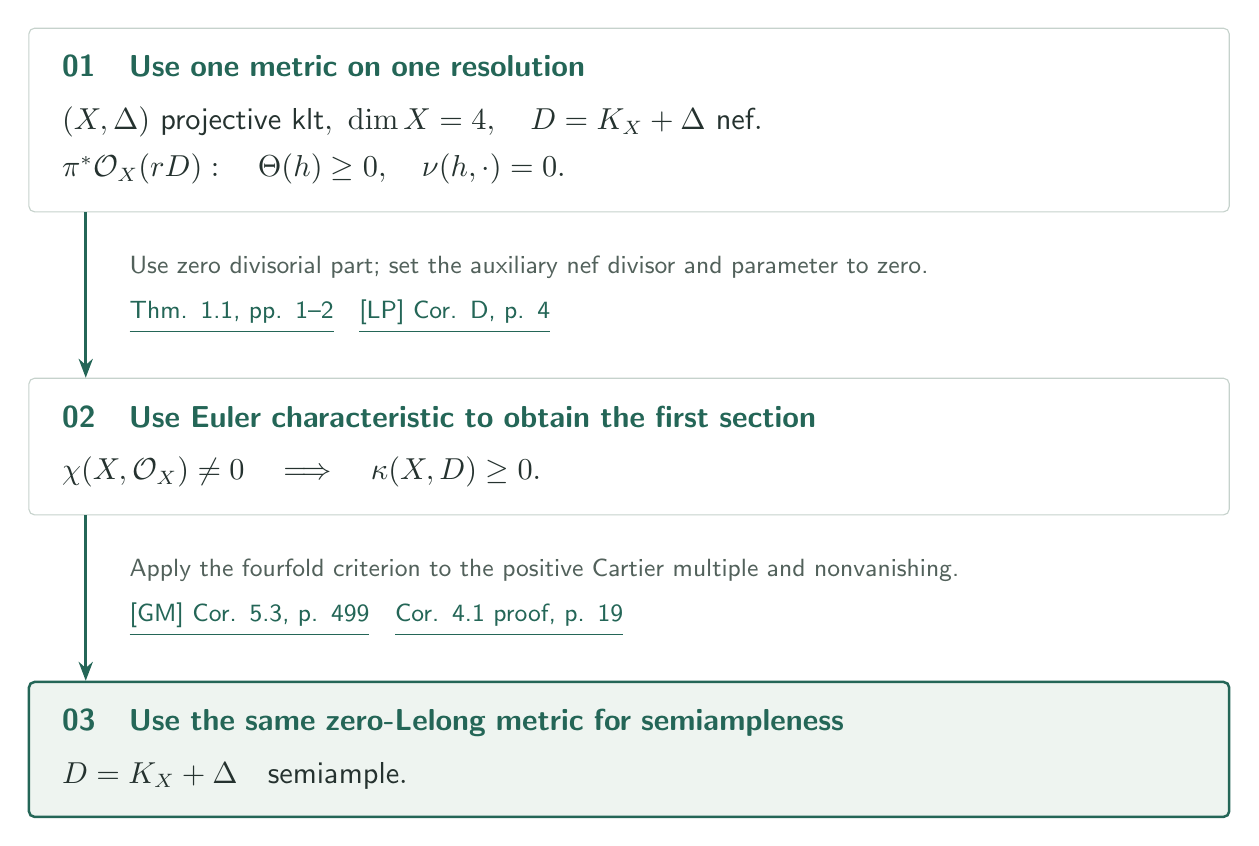
\begin{tikzpicture}
\node[card] (n0) {\heading{01}{同じ解消上の計量を用意する}{Use one metric on one resolution}\Tx{$(X,\Delta)\text{ projective klt},\ \dim X=4,\quad D=K_X+\Delta\text{ nef}.$\\[3pt]$\pi^*\mathcal O_X(rD):\quad \Theta(h)\ge0,\quad\nu(h,\cdot)=0.$}{$(X,\Delta)\text{ projective klt},\ \dim X=4,\quad D=K_X+\Delta\text{ nef}.$\\[3pt]$\pi^*\mathcal O_X(rD):\quad \Theta(h)\ge0,\quad\nu(h,\cdot)=0.$}};
\node[card,below=2.1cm of n0] (n1) {\heading{02}{Euler標数から最初の切断を得る}{Use Euler characteristic to obtain the first section}\Tx{$\chi(X,\mathcal O_X)\ne0\quad\Longrightarrow\quad\kappa(X,D)\ge0.$}{$\chi(X,\mathcal O_X)\ne0\quad\Longrightarrow\quad\kappa(X,D)\ge0.$}};
\flow{n0}{n1}{\Tx{一般化代数的特異点の因子部分を0とし、補助nef因子とパラメータを0にする。}{Use zero divisorial part; set the auxiliary nef divisor and parameter to zero.}\\[4pt]\Cite{mm}{Thm. 1.1, pp. 1--2}\quad \Cite{lp}{[LP] Cor. D, p. 4}}
\node[result,below=2.1cm of n1] (n2) {\heading{03}{同じ零Lelong数計量で半豊富性へ}{Use the same zero-Lelong metric for semiampleness}\Tx{$D=K_X+\Delta\quad\text{semiample}.$}{$D=K_X+\Delta\quad\text{semiample}.$}};
\flow{n1}{n2}{\Tx{正のCartier倍の計量と非負の小平次元を、四次元判定へ代入する。}{Apply the fourfold criterion to the positive Cartier multiple and nonvanishing.}\\[4pt]\Cite{gm}{[GM] Cor. 5.3, p. 499}\quad \Cite{mm}{Cor. 4.1 proof, p. 19}}
\end{tikzpicture}
\end{document}
